

\section{Corners}



\begin{frame}{Feature Extraction: Corners}
    \begin{figure}
      \centering
      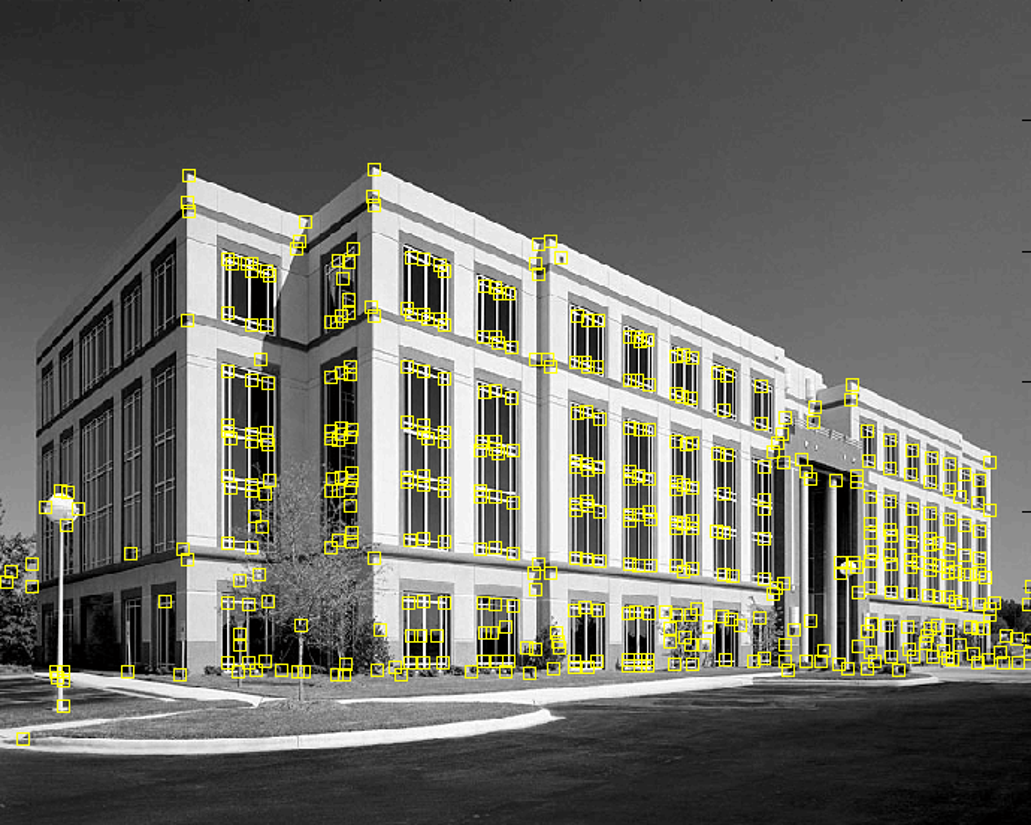
\includegraphics[width=0.7\textwidth]{harris_pkway.png}
      \caption{ Harris corners: 9300 Harris Corners Pkwy, Charlotte, NC}\label{fi:harris_pkway}
    \end{figure}
\end{frame}


\begin{frame}{Why Extract Features?}
    \begin{itemize}[<+->]
        \item Motivation: panorama stitching
        \item We have two images: how do we combine them?
    \end{itemize}
    \begin{columns}
        \column{0.8\textwidth}
        {
            \centering
            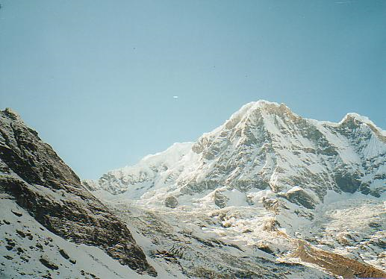
\includegraphics[width=0.45\textwidth]{img0000.png}
            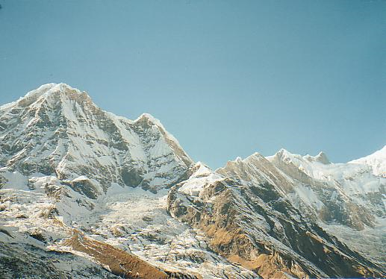
\includegraphics[width=0.45\textwidth]{img0001.png}
        }
        \column{0.2\textwidth}
        \begin{itemize}[<+->]
            \item[Step 1] Extract features.
            \item[Step 2] Match features.
            \item[Step 3] Align images.
        \end{itemize}
    \end{columns}
\end{frame}

\begin{frame}{Why Extract Features?}
    \begin{itemize}
        \item Motivation: panorama stitching
        \item We have two images: how do we combine them?
    \end{itemize}
    \begin{columns}
        \column{0.8\textwidth}
        {
            \centering
            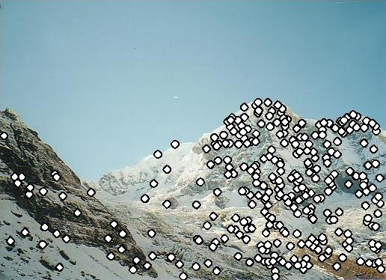
\includegraphics[width=0.45\textwidth]{img0003.png}
            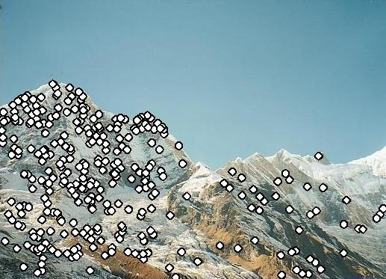
\includegraphics[width=0.45\textwidth]{img0002.png}
        }
        \column{0.2\textwidth}
        \begin{itemize}
            \item[Step 1] Extract features.
            \item[Step 2] Match features.
            \item[Step 3] Align images.
        \end{itemize}
    \end{columns}
\end{frame}

\begin{frame}
    \centering
    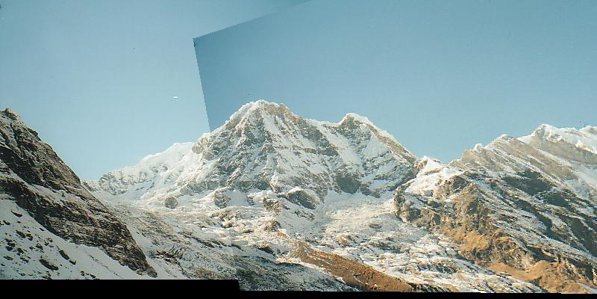
\includegraphics[width=0.8\textwidth]{img0004.png}
\end{frame}


\begin{frame}{Characteristics of Good Features}
    \begin{itemize}
        \item \alert{Repeatability}\\The same feature can be found in several images despite geometric and photometric transformations
        \item \alert{Saliency}\\Each feature is distinctive
        \item \alert{Compactness and efficiency}\\Many fewer features than image pixels
        \item \alert{Locality}\\A feature occupies a relatively small area of the image; robust to clutter and occlusion
    \end{itemize}
\end{frame}


\begin{frame}{Applications }
    Feature points are used for:
    \begin{itemize}
        \item Image alignment
        \item 3D reconstruction
        \item Motion tracking
        \item Robot navigation
        \item Indexing and database retrieval
        \item Object recognition
    \end{itemize}
    {
        \centering
        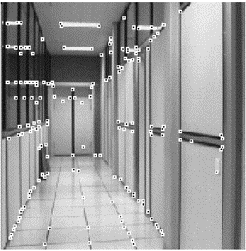
\includegraphics[width=0.3\textwidth]{img0005.png}
        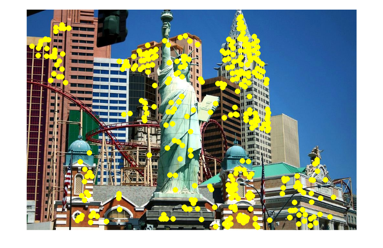
\includegraphics[width=0.3\textwidth]{img0006.png}
        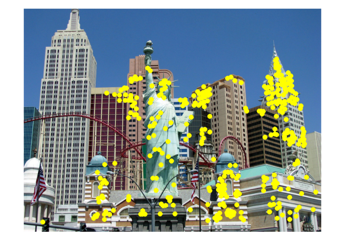
\includegraphics[width=0.3\textwidth]{img0007.png}
    }
\end{frame}
%
%
%\begin{frame}
%\frametitle{A Hard Feature Matching Problem}
%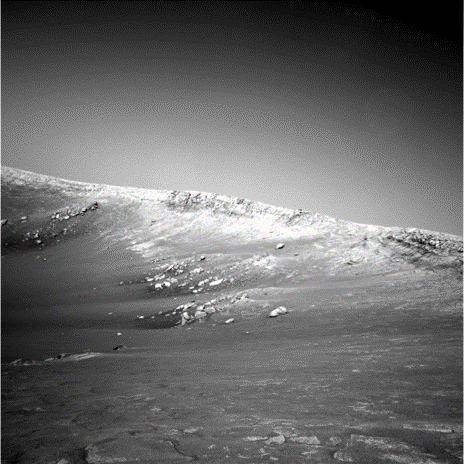
\includegraphics{img0008.png}
%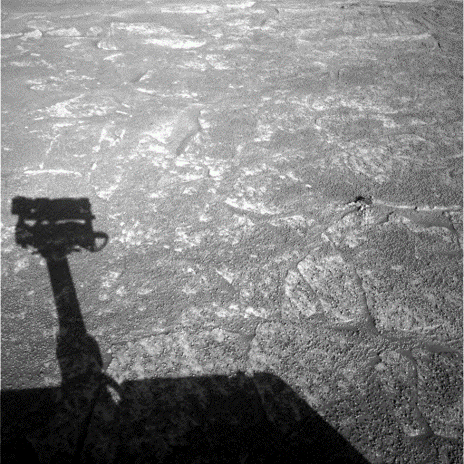
\includegraphics{img0009.png}
%\begin{itemize}
%\item NASA Mars Rover images
%\end{itemize}
%
%\end{frame}
%
%
%\begin{frame}
%\frametitle{Answer Below (look for tiny colored squares…)}
%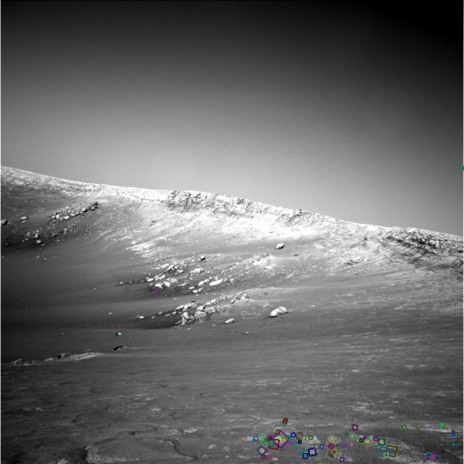
\includegraphics{img0010.png}
%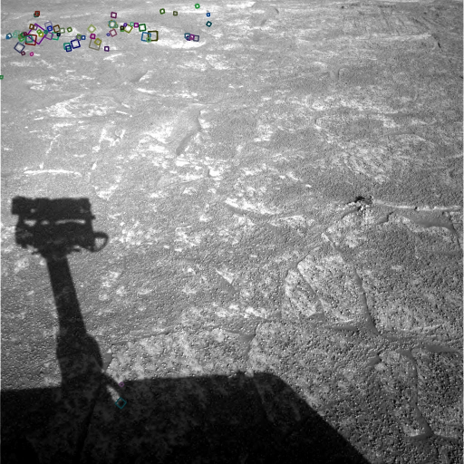
\includegraphics{img0011.png}
%\begin{itemize}
%\item NASA Mars Rover images
%\item with SIFT feature matches Figure by Noah Snavely
%\end{itemize}
%
%\end{frame}
%
%
%\begin{frame}
%\frametitle{Corner Detection: Basic Idea}
%\begin{itemize}
%\item We should easily recognize the point by looking through a small window
%\item Shifting a window in any direction should give a large change in intensity
%\end{itemize}
%%PartTitle: “edge”: no change along the edge direction
%%PartTitle:
%%PartTitle:
%%PartTitle: “corner”: significant change in all directions
%%PartTitle:
%%PartTitle:
%%PartTitle:
%%PartTitle:
%%PartTitle:
%%PartTitle: “flat” region: no change in all directions
%%PartTitle:
%%PartTitle:
%%PartTitle:
%%PartTitle:
%%PartTitle:
%
%\end{frame}
%
%
%\begin{frame}{Corner Detection: Mathematics}
%    \begin{itemize}
%        \item Change in appearance of window W for the shift [u,v]:
%    \end{itemize}
%    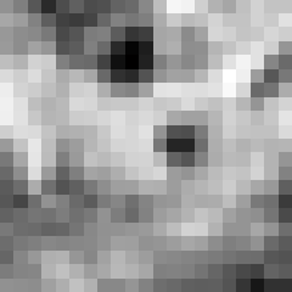
\includegraphics{img0012.png}
%    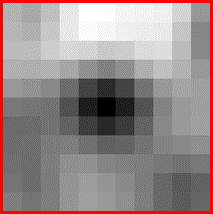
\includegraphics{img0013.png}
%    \begin{itemize}
%        \item I(x, y)
%    \end{itemize}
%    \begin{itemize}
%        \item E(u, v)
%    \end{itemize}
%    \begin{itemize}
%    \item E(3,2)
%    \end{itemize}
%    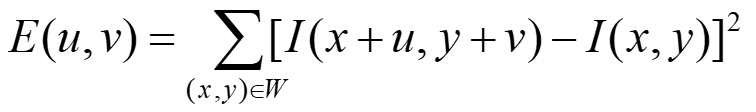
\includegraphics{img0014.png}
%
%\end{frame}
%
%
%\begin{frame}
%\frametitle{Corner Detection: Mathematics}
%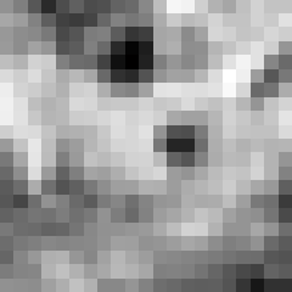
\includegraphics{img0015.png}
%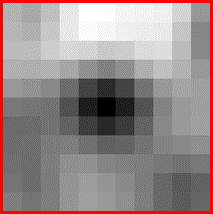
\includegraphics{img0016.png}
%\begin{itemize}
%\item I(x, y)
%\end{itemize}
%\begin{itemize}
%\item E(u, v)
%\end{itemize}
%\begin{itemize}
%\item E(0,0)
%\end{itemize}
%\begin{itemize}
%\item Change in appearance of window W for the shift [u,v]:
%\end{itemize}
%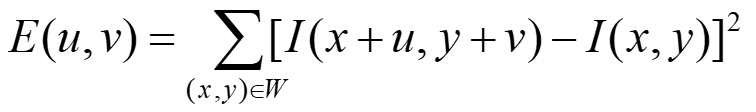
\includegraphics{img0017.png}
%
%\end{frame}
%
%
%\begin{frame}
%\frametitle{Corner Detection: Mathematics}
%\begin{itemize}
%\item We want to find out how this function behaves for small shifts
%\end{itemize}
%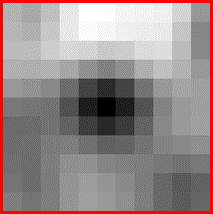
\includegraphics{img0018.png}
%\begin{itemize}
%\item E(u, v)
%\end{itemize}
%\begin{itemize}
%\item Change in appearance of window W for the shift [u,v]:
%\end{itemize}
%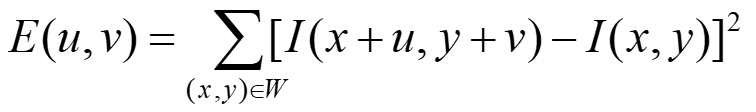
\includegraphics{img0019.png}
%
%\end{frame}
%
%
%\begin{frame}
%\frametitle{Corner Detection: Mathematics}
%\begin{itemize}
%\item First-order Taylor approximation for small motions [u, v]:
%\item
%\item
%\item Let’s plug this into E(u,v):
%\end{itemize}
%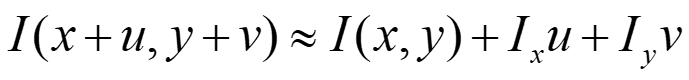
\includegraphics{img0020.png}
%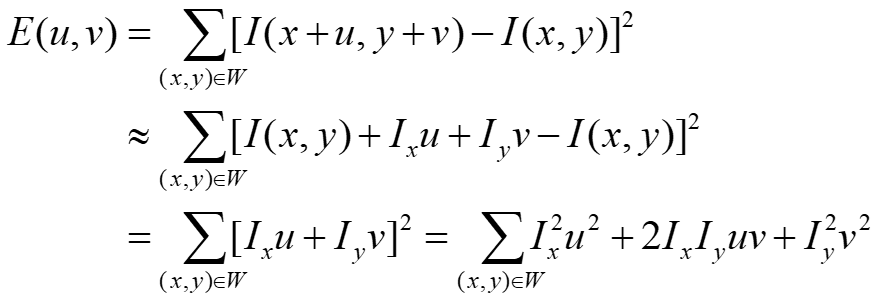
\includegraphics{img0021.png}
%
%\end{frame}
%
%
%\begin{frame}
%\frametitle{Corner Detection: Mathematics}
%\begin{itemize}
%\item The quadratic approximation can be written as
%\end{itemize}
%\begin{itemize}
%\item where M is a second moment matrix computed from image derivatives:
%\end{itemize}
%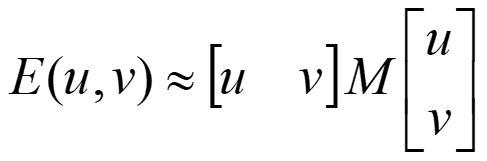
\includegraphics{img0022.png}
%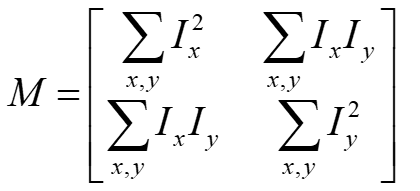
\includegraphics{img0023.png}
%\begin{itemize}
%\item (the sums are over all the pixels in the window W)
%\end{itemize}
%
%\end{frame}
%
%
%\begin{frame}
%\frametitle{Interpreting the Second Moment Matrix}
%\begin{itemize}
%\item The surface E(u,v) is locally approximated by a quadratic form. Let’s try to understand its shape.
%\begin{itemize}
%\item Specifically, in which directions does it have the smallest/greatest change?
%\end{itemize}
%\end{itemize}
%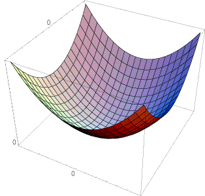
\includegraphics{img0024.png}
%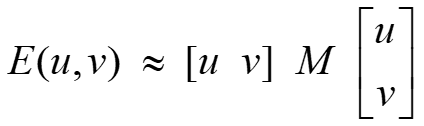
\includegraphics{img0025.png}
%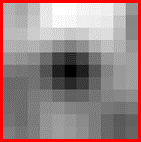
\includegraphics{img0026.png}
%\begin{itemize}
%\item E(u, v)
%\end{itemize}
%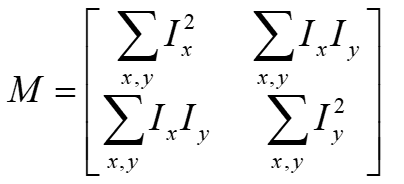
\includegraphics{img0027.png}
%
%\end{frame}
%
%
%\begin{frame}
%\frametitle{Interpreting the Second Moment Matrix}
%\begin{itemize}
%\item First, consider the axis-aligned case (gradients are either horizontal or vertical)
%\end{itemize}
%\begin{itemize}
%\item If either a or b is close to 0, then this is not a corner, so look for locations where both are large.
%\end{itemize}
%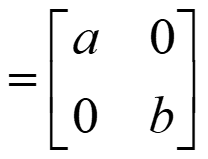
\includegraphics{img0028.png}
%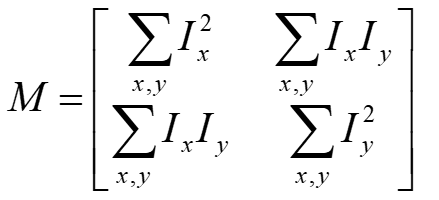
\includegraphics{img0029.png}
%
%\end{frame}
%
%
%\begin{frame}
%\frametitle{Interpreting the Second Moment Matrix}
%\begin{itemize}
%\item Consider a horizontal “slice” of E(u, v):
%\end{itemize}
%\begin{itemize}
%\item This is the equation of an ellipse.
%\end{itemize}
%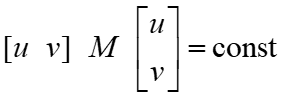
\includegraphics{img0030.png}
%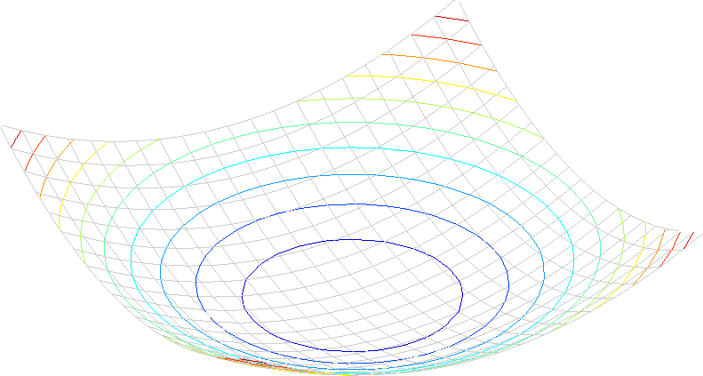
\includegraphics{img0031.png}
%
%\end{frame}
%
%
%\begin{frame}
%\frametitle{Interpreting the Second Moment Matrix}
%\begin{itemize}
%\item Consider a horizontal “slice” of E(u, v):
%\end{itemize}
%\begin{itemize}
%\item This is the equation of an ellipse.
%\end{itemize}
%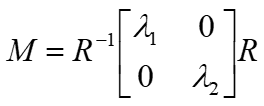
\includegraphics{img0032.png}
%\begin{itemize}
%\item The axis lengths of the ellipse are determined by the eigenvalues and the orientation is determined by R
%\end{itemize}
%%PartTitle: direction of the slowest change
%%PartTitle: direction of the fastest change
%%PartTitle:
%%PartTitle:
%%PartTitle:
%%PartTitle:
%%PartTitle:
%%PartTitle: (max)-1/2
%%PartTitle: (min)-1/2
%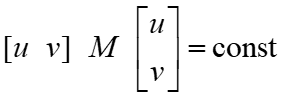
\includegraphics{img0033.png}
%\begin{itemize}
%\item Diagonalization of M:
%\end{itemize}
%
%\end{frame}
%
%
%\begin{frame}
%\frametitle{Visualization of Second Moment Matrices}
%
%\end{frame}
%
%
%\begin{frame}
%\frametitle{Visualization of Second Moment Matrices}
%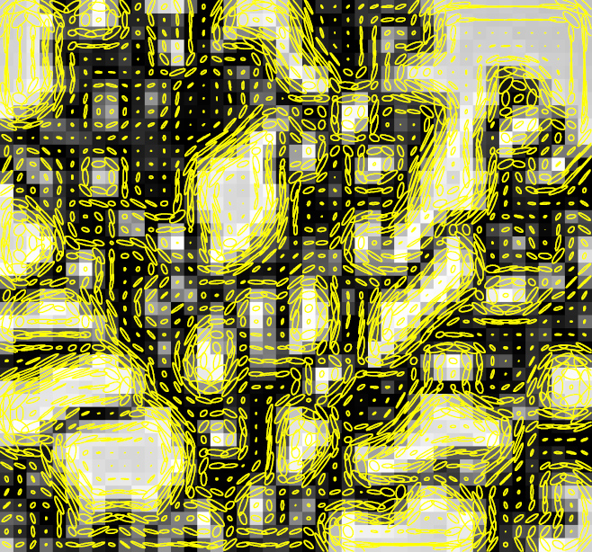
\includegraphics{img0034.png}
%
%\end{frame}
%
%
%\begin{frame}
%\frametitle{Interpreting the Eigenvalues}
%\begin{itemize}
%\item 1
%\end{itemize}
%\begin{itemize}
%\item 2
%\end{itemize}
%\begin{itemize}
%\item “Corner” 1 and 2 are large, 1 ~ 2;E increases in all directions
%\end{itemize}
%\begin{itemize}
%\item 1 and 2 are small; E is almost constant in all directions
%\end{itemize}
%\begin{itemize}
%\item “Edge” 1 >> 2
%\end{itemize}
%\begin{itemize}
%\item “Edge” 2 >> 1
%\end{itemize}
%\begin{itemize}
%\item “Flat” region
%\end{itemize}
%\begin{itemize}
%\item Classification of image points using eigenvalues of M:
%\end{itemize}
%
%\end{frame}
%
%
%\begin{frame}
%\frametitle{Corner Response Function}
%\begin{itemize}
%\item “Corner”R > 0
%\end{itemize}
%\begin{itemize}
%\item “Edge” R < 0
%\end{itemize}
%\begin{itemize}
%\item “Edge” R < 0
%\end{itemize}
%\begin{itemize}
%\item “Flat” region
%\end{itemize}
%\begin{itemize}
%\item |R| small
%\end{itemize}
%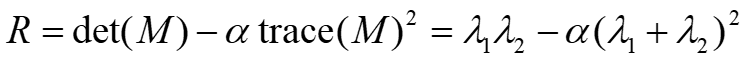
\includegraphics{img0035.png}
%\begin{itemize}
%\item α: constant (0.04 to 0.06)
%\end{itemize}
%
%\end{frame}
%
%
%\begin{frame}
%\frametitle{The Harris Corner Detector}
%\begin{itemize}
%\item Compute partial derivatives at each pixel
%\item Compute second moment matrix M in a Gaussian window around each pixel:
%\end{itemize}
%\begin{itemize}
%\item C.Harris and M.Stephens. “A Combined Corner and Edge Detector.” Proceedings of the 4th Alvey Vision Conference: pages 147—151, 1988. 
%\end{itemize}
%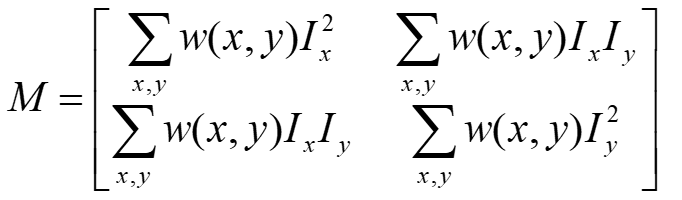
\includegraphics{img0036.png}
%
%\end{frame}
%
%
%\begin{frame}
%\frametitle{The Harris Corner Detector}
%\begin{itemize}
%\item Compute partial derivatives at each pixel
%\item Compute second moment matrix M in a Gaussian window around each pixel
%\item Compute corner response function R
%\end{itemize}
%\begin{itemize}
%\item C.Harris and M.Stephens. “A Combined Corner and Edge Detector.” Proceedings of the 4th Alvey Vision Conference: pages 147—151, 1988. 
%\end{itemize}
%
%\end{frame}
%
%
%\begin{frame}
%\frametitle{Harris Detector: Steps}
%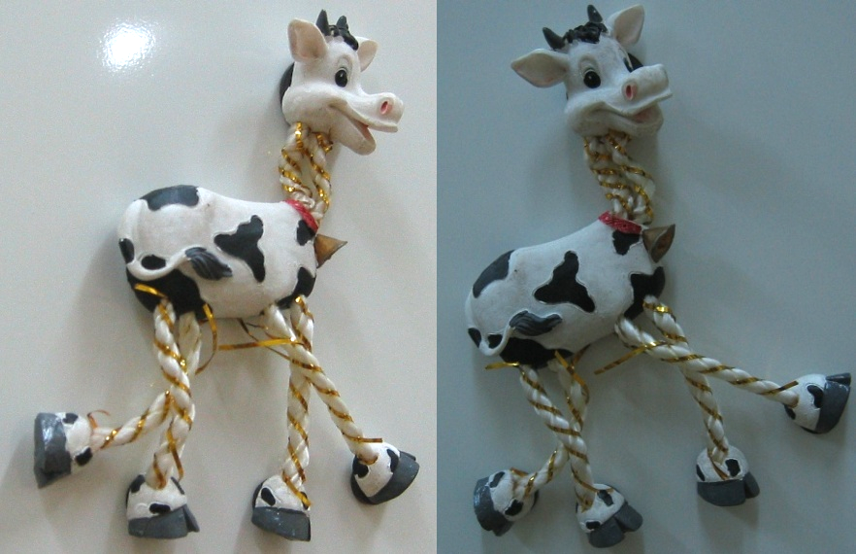
\includegraphics{img0037.png}
%
%\end{frame}
%
%
%\begin{frame}
%\frametitle{Harris Detector: Steps}
%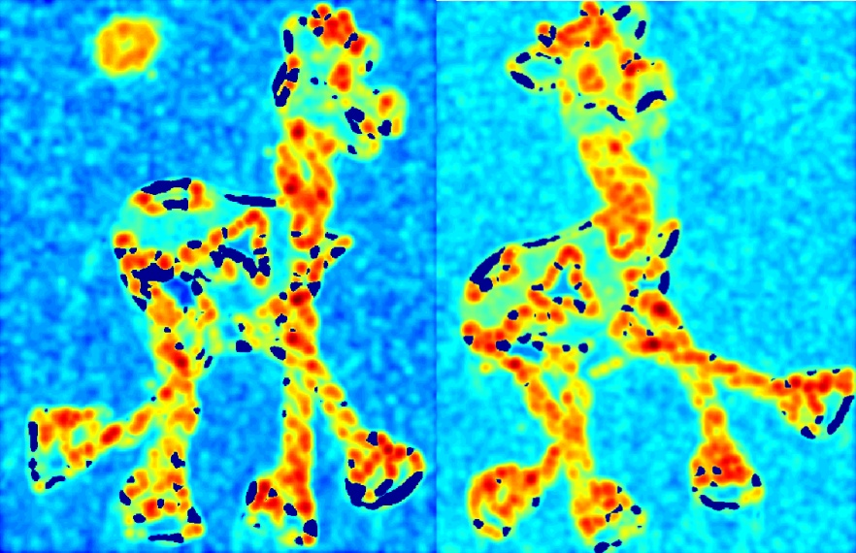
\includegraphics{img0038.png}
%\begin{itemize}
%\item Compute corner response R
%\end{itemize}
%
%\end{frame}
%
%
%\begin{frame}
%\frametitle{The Harris Corner Detector}
%\begin{itemize}
%\item Compute partial derivatives at each pixel
%\item Compute second moment matrix M in a Gaussian window around each pixel
%\item Compute corner response function R
%\item Threshold R
%\item Find local maxima of response function (nonmaximum suppression)
%\end{itemize}
%\begin{itemize}
%\item C.Harris and M.Stephens. “A Combined Corner and Edge Detector.” Proceedings of the 4th Alvey Vision Conference: pages 147—151, 1988. 
%\end{itemize}
%
%\end{frame}
%
%
%\begin{frame}
%\frametitle{Harris Detector: Steps}
%\begin{itemize}
%\item Find points with large corner response: R > threshold
%\end{itemize}
%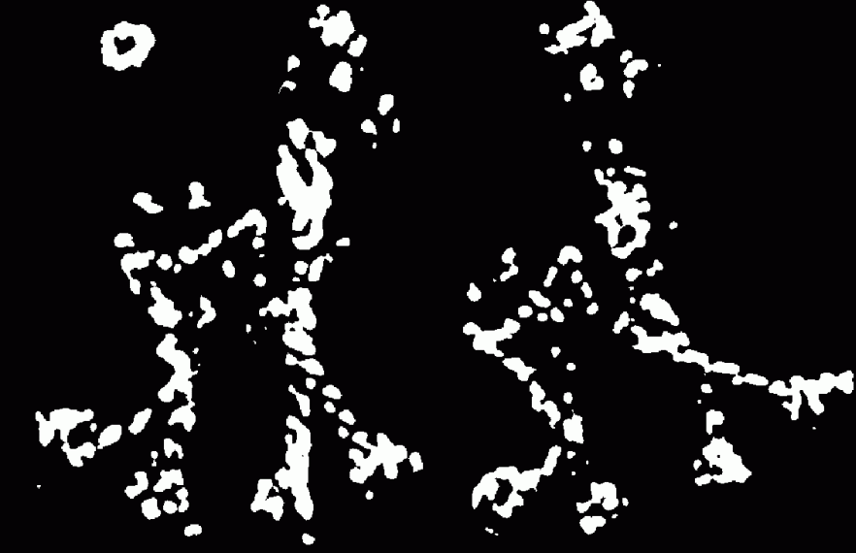
\includegraphics{img0039.png}
%
%\end{frame}
%
%
%\begin{frame}
%\frametitle{Harris Detector: Steps}
%\begin{itemize}
%\item Take only the points of local maxima of R
%\end{itemize}
%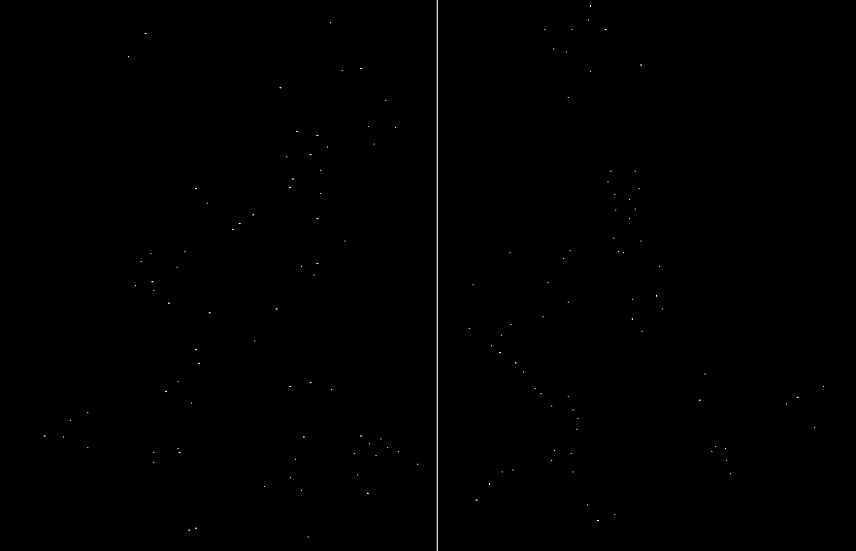
\includegraphics{img0040.png}
%
%\end{frame}
%
%
%\begin{frame}
%\frametitle{Harris Detector: Steps}
%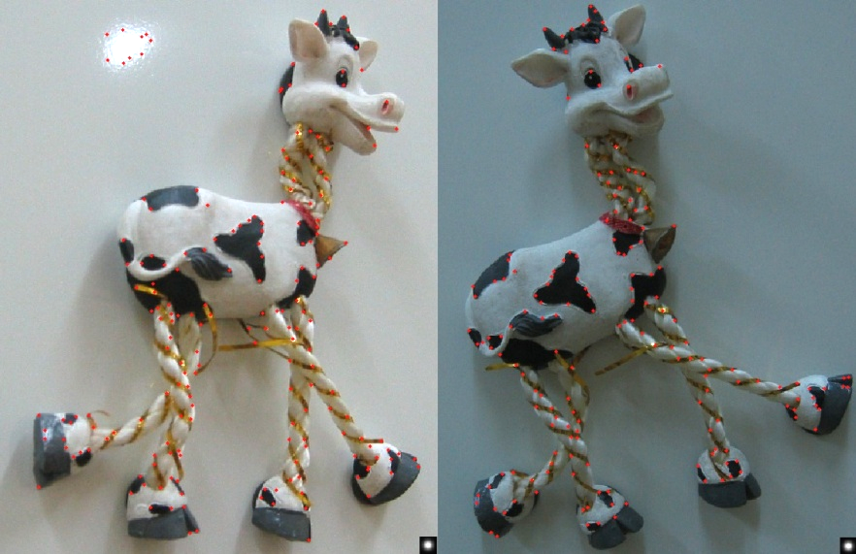
\includegraphics{img0041.png}
%
%\end{frame}
%
%
%\begin{frame}
%\frametitle{Invariance and Covariance}
%\begin{itemize}
%\item We want corner locations to be invariant to photometric transformations and covariant to geometric transformations
%\begin{itemize}
%\item Invariance: image is transformed and corner locations do not change
%\item Covariance: if we have two transformed versions of the same image, features should be detected in corresponding locations
%\end{itemize}
%\end{itemize}
%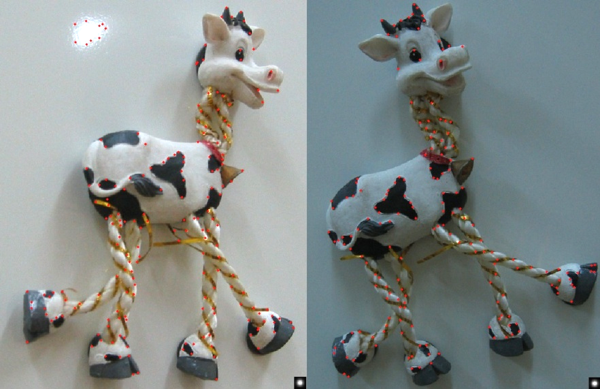
\includegraphics{img0042.png}
%
%\end{frame}
%
%
%\begin{frame}
%\frametitle{Activity}
%\begin{itemize}
%\item Discuss in pairs and decide:
%\item I may randomly ask a pair to respond.
%\item Is Harris corner detection invariant to
%\item Affine intensity changes
%\item  Image translation
%\item Image rotation
%\item Image scaling
%\end{itemize}
%\begin{itemize}
%\item I  a I + b
%\end{itemize}
%
%\end{frame}
%
%
%\begin{frame}
%\frametitle{Affine Intensity Change}
%\begin{itemize}
%\item    Only derivatives are used => invariance to intensity shift I  I + b
%\end{itemize}
%%PartTitle:    Intensity scaling: I  a I
%%PartTitle:
%%PartTitle:
%%PartTitle:
%%PartTitle:
%%PartTitle: R
%%PartTitle: x (image coordinate)
%%PartTitle:
%%PartTitle: threshold
%%PartTitle:
%%PartTitle:
%%PartTitle: R
%%PartTitle: x (image coordinate)
%%PartTitle:
%%PartTitle:
%%PartTitle:
%%PartTitle:
%%PartTitle:
%%PartTitle:
%%PartTitle:
%%PartTitle:
%\begin{itemize}
%\item Partially invariant to affine intensity change
%\end{itemize}
%\begin{itemize}
%\item I  a I + b
%\end{itemize}
%
%\end{frame}
%
%
%\begin{frame}
%\frametitle{Image Translation}
%\begin{itemize}
%\item   Derivatives and window function are shift-invariant
%\end{itemize}
%\begin{itemize}
%\item Corner location is covariant w.r.t. translation
%\end{itemize}
%
%\end{frame}
%
%
%\begin{frame}
%\frametitle{Image Rotation}
%\begin{itemize}
%\item Second moment ellipse rotates but its shape (i.e. eigenvalues) remains the same
%\end{itemize}
%%PartTitle:
%%PartTitle:
%%PartTitle:
%%PartTitle:
%%PartTitle:
%%PartTitle:
%%PartTitle:
%%PartTitle:
%%PartTitle:
%%PartTitle:
%%PartTitle:
%\begin{itemize}
%\item Corner location is covariant w.r.t. rotation
%\end{itemize}
%
%\end{frame}
%
%
%\begin{frame}
%\frametitle{Scaling}
%\begin{itemize}
%\item All points will be classified as edges
%\end{itemize}
%%PartTitle:
%%PartTitle:
%\begin{itemize}
%\item Corner
%\end{itemize}
%\begin{itemize}
%\item Corner location is not covariant to scaling!
%\end{itemize}
%%PartTitle:
%%PartTitle:
%%PartTitle:
%%PartTitle:
%%PartTitle:
%
%\end{frame}
%
%
%\begin{frame}
%\frametitle{BLOB DETECTION}
%\begin{itemize}
%\item Slides from Svetlana Lazebnik
%\end{itemize}
%
%\end{frame}
%
%
%\begin{frame}
%\frametitle{Blob Detection}
%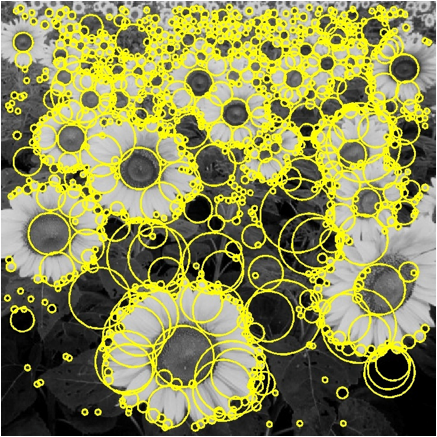
\includegraphics{img0043.png}
%
%\end{frame}
%
%
%\begin{frame}
%\frametitle{Feature Detection with Scale Selection}
%\begin{itemize}
%\item We want to extract features with characteristic scale that is covariant with the image transformation
%\end{itemize}
%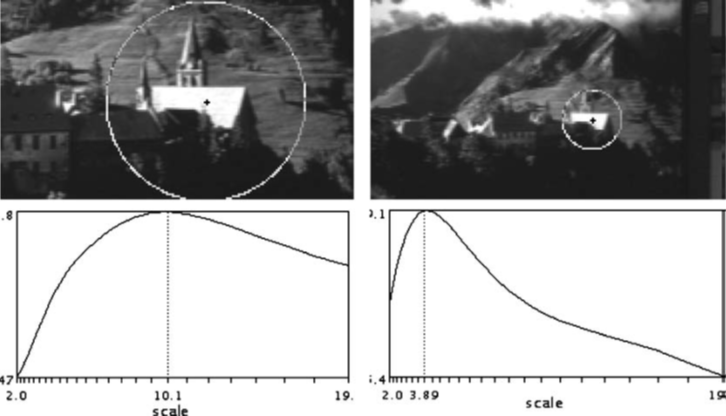
\includegraphics{img0044.png}
%
%\end{frame}
%
%
%\begin{frame}
%\frametitle{Blob Detection: Basic idea}
%\begin{itemize}
%\item To detect blobs, convolve the image with a “blob filter” at multiple scales and look for extrema of filter response in the resulting scale space.
%\end{itemize}
%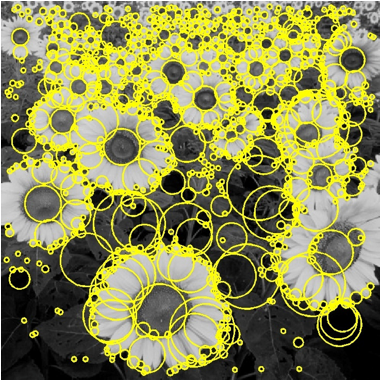
\includegraphics{img0045.png}
%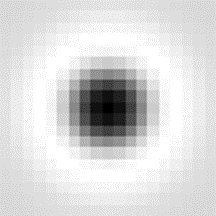
\includegraphics{img0046.png}
%
%\end{frame}
%
%
%\begin{frame}
%\frametitle{Blob Detection: Basic Idea}
%\begin{itemize}
%\item Find maxima and minima of blob filter response in space and scale
%\end{itemize}
%
\includegraphics{img0047.png}
%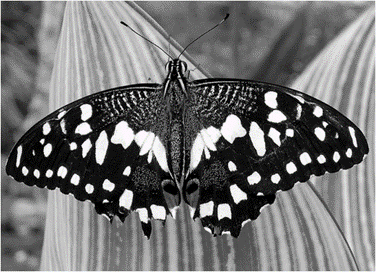
\includegraphics{img0048.png}
%\includegraphics{img0049.png}
%\begin{itemize}
%\item *
%\end{itemize}
%\begin{itemize}
%\item =
%\end{itemize}
%\begin{itemize}
%\item maxima
%\end{itemize}
%\begin{itemize}
%\item minima
%\end{itemize}
%\begin{itemize}
%\item Source: N. Snavely
%\end{itemize}
%
%\end{frame}
%
%
%\begin{frame}
%\frametitle{Blob Filter}
%\begin{itemize}
%\item Laplacian of Gaussian: Circularly symmetric operator for blob detection in 2D
%\end{itemize}
%\includegraphics{img0050.png}
%\includegraphics{img0051.png}
%\includegraphics{img0052.png}
%
%\end{frame}
%
%
%\begin{frame}
%\frametitle{Recall: Edge Detection}
%\includegraphics{img0053.png}
%\begin{itemize}
%\item f
%\end{itemize}
%\includegraphics{img0054.png}
%\begin{itemize}
%\item Source: S. Seitz
%\end{itemize}
%\begin{itemize}
%\item Edge
%\end{itemize}
%\begin{itemize}
%\item Derivative of Gaussian
%\end{itemize}
%\begin{itemize}
%\item Edge = maximum of derivative
%\end{itemize}
%
%\end{frame}
%
%
%\begin{frame}
%\frametitle{Edge Detection, Take 2}
%\includegraphics{img0055.png}
%\begin{itemize}
%\item f
%\end{itemize}
%\includegraphics{img0056.png}
%\begin{itemize}
%\item Edge
%\end{itemize}
%\begin{itemize}
%\item Second derivative of Gaussian (Laplacian)
%\end{itemize}
%\begin{itemize}
%\item Edge = zero crossing of second derivative
%\end{itemize}
%\begin{itemize}
%\item Source: S. Seitz
%\end{itemize}
%
%\end{frame}
%
%
%\begin{frame}
%\frametitle{From Edges to Blobs}
%\includegraphics{img0057.png}
%\begin{itemize}
%\item Edge = ripple
%\item Blob = superposition of two ripples
%\end{itemize}
%\begin{itemize}
%\item Spatial selection: the magnitude of the Laplacian response will achieve a maximum at the center of the blob, provided the scale of the Laplacian is “matched” to the scale of the blob
%\end{itemize}
%%PartTitle: maximum
%%PartTitle:
%
%\end{frame}
%
%
%\begin{frame}
%\frametitle{Scale Selection}
%\begin{itemize}
%\item We want to find the characteristic scale of the blob by convolving it with Laplacians at several scales and looking for the maximum response
%\item However, Laplacian response decays as scale increases:
%\end{itemize}
%%PartTitle: increasing σ
%%PartTitle:
%%PartTitle: original signal (radius=8)
%
%\end{frame}
%
%
%\begin{frame}
%\frametitle{Scale Normalization}
%\begin{itemize}
%\item The response of a derivative of Gaussian filter to a perfect step edge decreases as σ increases
%\end{itemize}
%\includegraphics{img0058.png}
%\includegraphics{img0059.png}
%
%\end{frame}
%
%
%\begin{frame}
%\frametitle{Scale Normalization}
%\begin{itemize}
%\item The response of a derivative of Gaussian filter to a perfect step edge decreases as σ increases
%\item To keep response the same (scale-invariant), must multiply Gaussian derivative by σ
%\item Laplacian is the second Gaussian derivative, so it must be multiplied by σ2
%\end{itemize}
%
%\end{frame}
%
%
%\begin{frame}
%\frametitle{Effect of Scale Normalization}
%%PartTitle: Scale-normalized Laplacian response
%\includegraphics{img0060.png}
%\begin{itemize}
%\item Unnormalized Laplacian response
%\end{itemize}
%\begin{itemize}
%\item Original signal
%\end{itemize}
%%PartTitle: maximum
%%PartTitle:
%
%\end{frame}
%
%
%\begin{frame}
%\frametitle{Blob Detection in 2D}
%\begin{itemize}
%\item Laplacian of Gaussian: Circularly symmetric operator for blob detection in 2D
%\end{itemize}
%\includegraphics{img0061.png}
%\includegraphics{img0062.png}
%\includegraphics{img0063.png}
%\begin{itemize}
%\item Scale-normalized:
%\end{itemize}
%
%\end{frame}
%
%
%\begin{frame}
%\frametitle{Scale Selection}
%\begin{itemize}
%\item At what scale does the Laplacian achieve a maximum response to a binary circle of radius r?
%\end{itemize}
%\begin{itemize}
%\item r
%\end{itemize}
%\begin{itemize}
%\item image
%\end{itemize}
%\includegraphics{img0064.png}
%\includegraphics{img0065.png}
%\begin{itemize}
%\item Laplacian
%\end{itemize}
%
%\end{frame}
%
%
%\begin{frame}
%\frametitle{Scale Selection}
%\begin{itemize}
%\item At what scale does the Laplacian achieve a maximum response to a binary circle of radius r?
%\item To get maximum response, the zeros of the Laplacian have to be aligned with the circle
%\item The Laplacian is given by (up to scale):
%\item Therefore, the maximum response occurs at
%\item
%\end{itemize}
%\begin{itemize}
%\item r
%\end{itemize}
%\begin{itemize}
%\item image
%\end{itemize}
%\includegraphics{img0066.png}
%\includegraphics{img0067.png}
%%PartTitle:
%%PartTitle:
%%PartTitle: circle
%%PartTitle: Laplacian
%\begin{itemize}
%\item 0
%\end{itemize}
%
%\end{frame}
%
%
%\begin{frame}
%\frametitle{Characteristic Scale}
%\begin{itemize}
%\item We define the characteristic scale of a blob as the scale that produces peak of Laplacian response in the blob center
%\end{itemize}
%%PartTitle:
%\begin{itemize}
%\item characteristic scale
%\end{itemize}
%\begin{itemize}
%\item T. Lindeberg (1998). "Feature detection with automatic scale selection." International Journal of Computer Vision 30 (2): pp 77--116.
%\end{itemize}
%
%\end{frame}
%
%
%\begin{frame}
%\frametitle{Scale-Space Blob Detector}
%\begin{itemize}
%\item Convolve image with scale-normalized Laplacian at several scales
%\end{itemize}
%
%\end{frame}
%
%
%\begin{frame}
%\frametitle{Scale-Space Blob Detector: Example}
%\includegraphics{img0068.png}
%
%\end{frame}
%
%
%\begin{frame}
%\frametitle{Scale-Space Blob Detector: Example}
%\includegraphics{img0069.png}
%\includegraphics{img0070.png}
%\includegraphics{img0071.png}
%\includegraphics{img0072.png}
%\includegraphics{img0073.png}
%\includegraphics{img0074.png}
%\includegraphics{img0075.png}
%\includegraphics{img0076.png}
%\includegraphics{img0077.png}
%\includegraphics{img0078.png}
%
%\end{frame}
%
%
%\begin{frame}
%\frametitle{Scale-Space Blob Detector}
%\begin{itemize}
%\item Convolve image with scale-normalized Laplacian at several scales
%\item Find maxima of squared Laplacian response in scale-space
%\end{itemize}
%\includegraphics{img0079.png}
%
%\end{frame}
%
%
%\begin{frame}
%\frametitle{Scale-Space Blob Detector: Example}
%\includegraphics{img0080.png}
%
%\end{frame}
%
%
%\begin{frame}
%\frametitle{Efficient Implementation}
%\begin{itemize}
%\item Approximating the Laplacian with a difference of Gaussians:
%\end{itemize}
%\includegraphics{img0081.png}
%\begin{itemize}
%\item (Laplacian)
%\end{itemize}
%\begin{itemize}
%\item (Difference of Gaussians)
%\end{itemize}
%
%\end{frame}
%
%
%\begin{frame}
%\frametitle{Efficient Implementation}
%\begin{itemize}
%\item David G. Lowe. "Distinctive image features from scale-invariant keypoints.” IJCV 60 (2), pp. 91-110, 2004.
%\end{itemize}
%
%\end{frame}
%
%
%\begin{frame}
%\frametitle{From Feature Detection to Feature Description}
%\begin{itemize}
%\item Scaled and rotated versions of the same neighborhood will give rise to blobs that are related by the same transformation
%\item What to do if we want to compare the appearance of these image regions?
%\begin{itemize}
%\item Normalization: transform these regions into same-size circles
%\item Problem: rotational ambiguity
%\end{itemize}
%\end{itemize}
%%PartTitle:
%%PartTitle:
%\includegraphics{img0082.png}
%\includegraphics{img0083.png}
%
%\end{frame}
%
%
%\begin{frame}
%\frametitle{Eliminating Rotation Ambiguity}
%\begin{itemize}
%\item To assign a unique orientation to circular image windows:
%\begin{itemize}
%\item Create histogram of local gradient directions in the patch
%\item Assign canonical orientation at peak of smoothed histogram
%\end{itemize}
%\end{itemize}
%\includegraphics{img0084.png}
%%PartTitle:
%%PartTitle:
%%PartTitle:
%%PartTitle:
%%PartTitle:
%%PartTitle:
%%PartTitle:
%%PartTitle:
%%PartTitle:
%%PartTitle:
%%PartTitle:
%%PartTitle:
%%PartTitle:
%%PartTitle:
%%PartTitle:
%%PartTitle:
%%PartTitle:
%%PartTitle:
%%PartTitle:
%%PartTitle:
%%PartTitle:
%%PartTitle:
%%PartTitle:
%%PartTitle:
%%PartTitle:
%%PartTitle:
%%PartTitle:
%%PartTitle:
%%PartTitle:
%%PartTitle:
%%PartTitle:
%%PartTitle:
%%PartTitle:
%%PartTitle:
%%PartTitle:
%%PartTitle:
%%PartTitle:
%%PartTitle:
%%PartTitle:
%%PartTitle: 0
%%PartTitle: 2
%%PartTitle: p
%%PartTitle:
%%PartTitle:
%%PartTitle:
%
%\end{frame}
%
%
%\begin{frame}
%\frametitle{SIFT Features}
%\begin{itemize}
%\item Detected features with characteristic scales and orientations:
%\end{itemize}
%\includegraphics{img0085.png}
%\begin{itemize}
%\item David G. Lowe. "Distinctive image features from scale-invariant keypoints.” IJCV 60 (2), pp. 91-110, 2004.
%\end{itemize}
%\includegraphics{img0086.png}
%
%\end{frame}
%
%
%\begin{frame}
%\frametitle{From Feature Detection to Feature Description}
%\begin{itemize}
%\item Detection is covariant:
%\begin{itemize}
%\item 	features(transform(image)) = transform(features(image))
%\end{itemize}
%\item Description is invariant:
%\begin{itemize}
%\item 	features(transform(image)) = features(image)
%\end{itemize}
%\end{itemize}
%\includegraphics{img0087.png}
%
%\end{frame}
%
%
%\begin{frame}
%\frametitle{SIFT Descriptors}
%\includegraphics{img0088.png}
%\begin{itemize}
%\item David G. Lowe. "Distinctive image features from scale-invariant keypoints.” IJCV 60 (2), pp. 91-110, 2004.
%\end{itemize}
%
%\end{frame}
%
%
%\begin{frame}
%\frametitle{Properties of SIFT}
%\begin{itemize}
%\item Extraordinarily robust detection and description technique
%\begin{itemize}
%\item Can handle changes in viewpoint
%\begin{itemize}
%\item Up to about 60 degree out-of-plane rotation
%\end{itemize}
%\item Can handle significant changes in illumination
%\begin{itemize}
%\item Sometimes even day vs. night
%\end{itemize}
%\item Fast and efficient—can run in real time
%\item Lots of code available
%\end{itemize}
%\end{itemize}
%\includegraphics{img0089.png}
%\includegraphics{img0090.png}
%\begin{itemize}
%\item Source: N. Snavely
%\end{itemize}
%
%\end{frame}
%
%
%\begin{frame}
%\frametitle{Affine adaptation}
%\begin{itemize}
%\item Affine transformation approximates viewpoint changes for roughly planar objects and roughly orthographic cameras
%\end{itemize}
%\includegraphics{img0091.png}
%\includegraphics{img0092.png}
%
%\end{frame}
%
%
%\begin{frame}
%\frametitle{Affine Adaptation}
%\includegraphics{img0093.png}
%%PartTitle: direction of the slowest change
%%PartTitle: direction of the fastest change
%%PartTitle:
%%PartTitle:
%%PartTitle:
%%PartTitle:
%%PartTitle:
%%PartTitle: (max)-1/2
%%PartTitle: (min)-1/2
%\begin{itemize}
%\item Consider the second moment matrix of the window containing the blob:
%\end{itemize}
%\includegraphics{img0094.png}
%\begin{itemize}
%\item Recall:
%\end{itemize}
%\begin{itemize}
%\item This ellipse visualizes the “characteristic shape” of the window
%\end{itemize}
%
%\end{frame}
%
%
%\begin{frame}
%\frametitle{Affine Adaptation Example}
%\includegraphics{img0095.png}
%\begin{itemize}
%\item Scale-invariant regions (blobs)
%\end{itemize}
%
%\end{frame}
%
%
%\begin{frame}
%\frametitle{Affine Adaptation Example}
%\includegraphics{img0096.png}
%\begin{itemize}
%\item Affine-adapted blobs
%\end{itemize}
%
%\end{frame} 